\documentclass{article}

\usepackage[a4paper]{geometry}
\usepackage[T1]{fontenc}
\usepackage{graphicx}
\usepackage{amsmath}
\usepackage{amssymb}
\usepackage{listings}
\usepackage{xcolor}
\usepackage{booktabs}
\usepackage{parskip}
\usepackage{float}
\usepackage{wrapfig}

\definecolor{gb_black}{HTML}{282828}
\definecolor{gb_gray}{HTML}{928374}
\definecolor{gb_red}{HTML}{cc241d}
\definecolor{gb_green}{HTML}{98971a}
\definecolor{gb_blue}{HTML}{458588}
\colorlet{background-color}{gb_gray!5}

\lstset{
    basicstyle=\color{gb_black}\ttfamily,
    keywordstyle=\color{gb_red},
    commentstyle=\color{gb_blue},
    stringstyle=\color{gb_green},
    numberstyle=\color{gb_black!35}\ttfamily,
    showspaces=false,
    showstringspaces=false,
    showtabs=false,
    columns=fullflexible,
    breaklines=true,
    postbreak=\mbox{\textcolor{gb_gray}{\(\hookrightarrow\)}\space},
    escapechar=\$,
    backgroundcolor=\color{background-color},
    numbers=none,
    frame=single,
    framerule=0pt,
}

% change the default enumeration style to alphabetic with parentheses
% \renewcommand{\theenumi}{\alph{enumi}}
% \renewcommand{\labelenumi}{(\theenumi)}

\title{ECM2419: Software Development Coursework}
\author{730022096 \& 730002704}
\date{}

\begin{document}

\maketitle
\tableofcontents
\section*{Declaration}
No GenAI was used in the production of this report or the associated code.

\clearpage

\section{Design Choices} % Max two pages
\subsection{The V-Model}
We chose to use the V-Model of software development as our software engineering lifecycle. This model is characterised by the planning, preparation, and documentation phases being completed before any code is written. This model has five phases: feasibility, design, implementation, testing, and maintenance. Because of the nature of our project, we can ignore the feasibility and maintenance phases.

\begin{wrapfigure}{r}{0.55\textwidth}
    \centering
    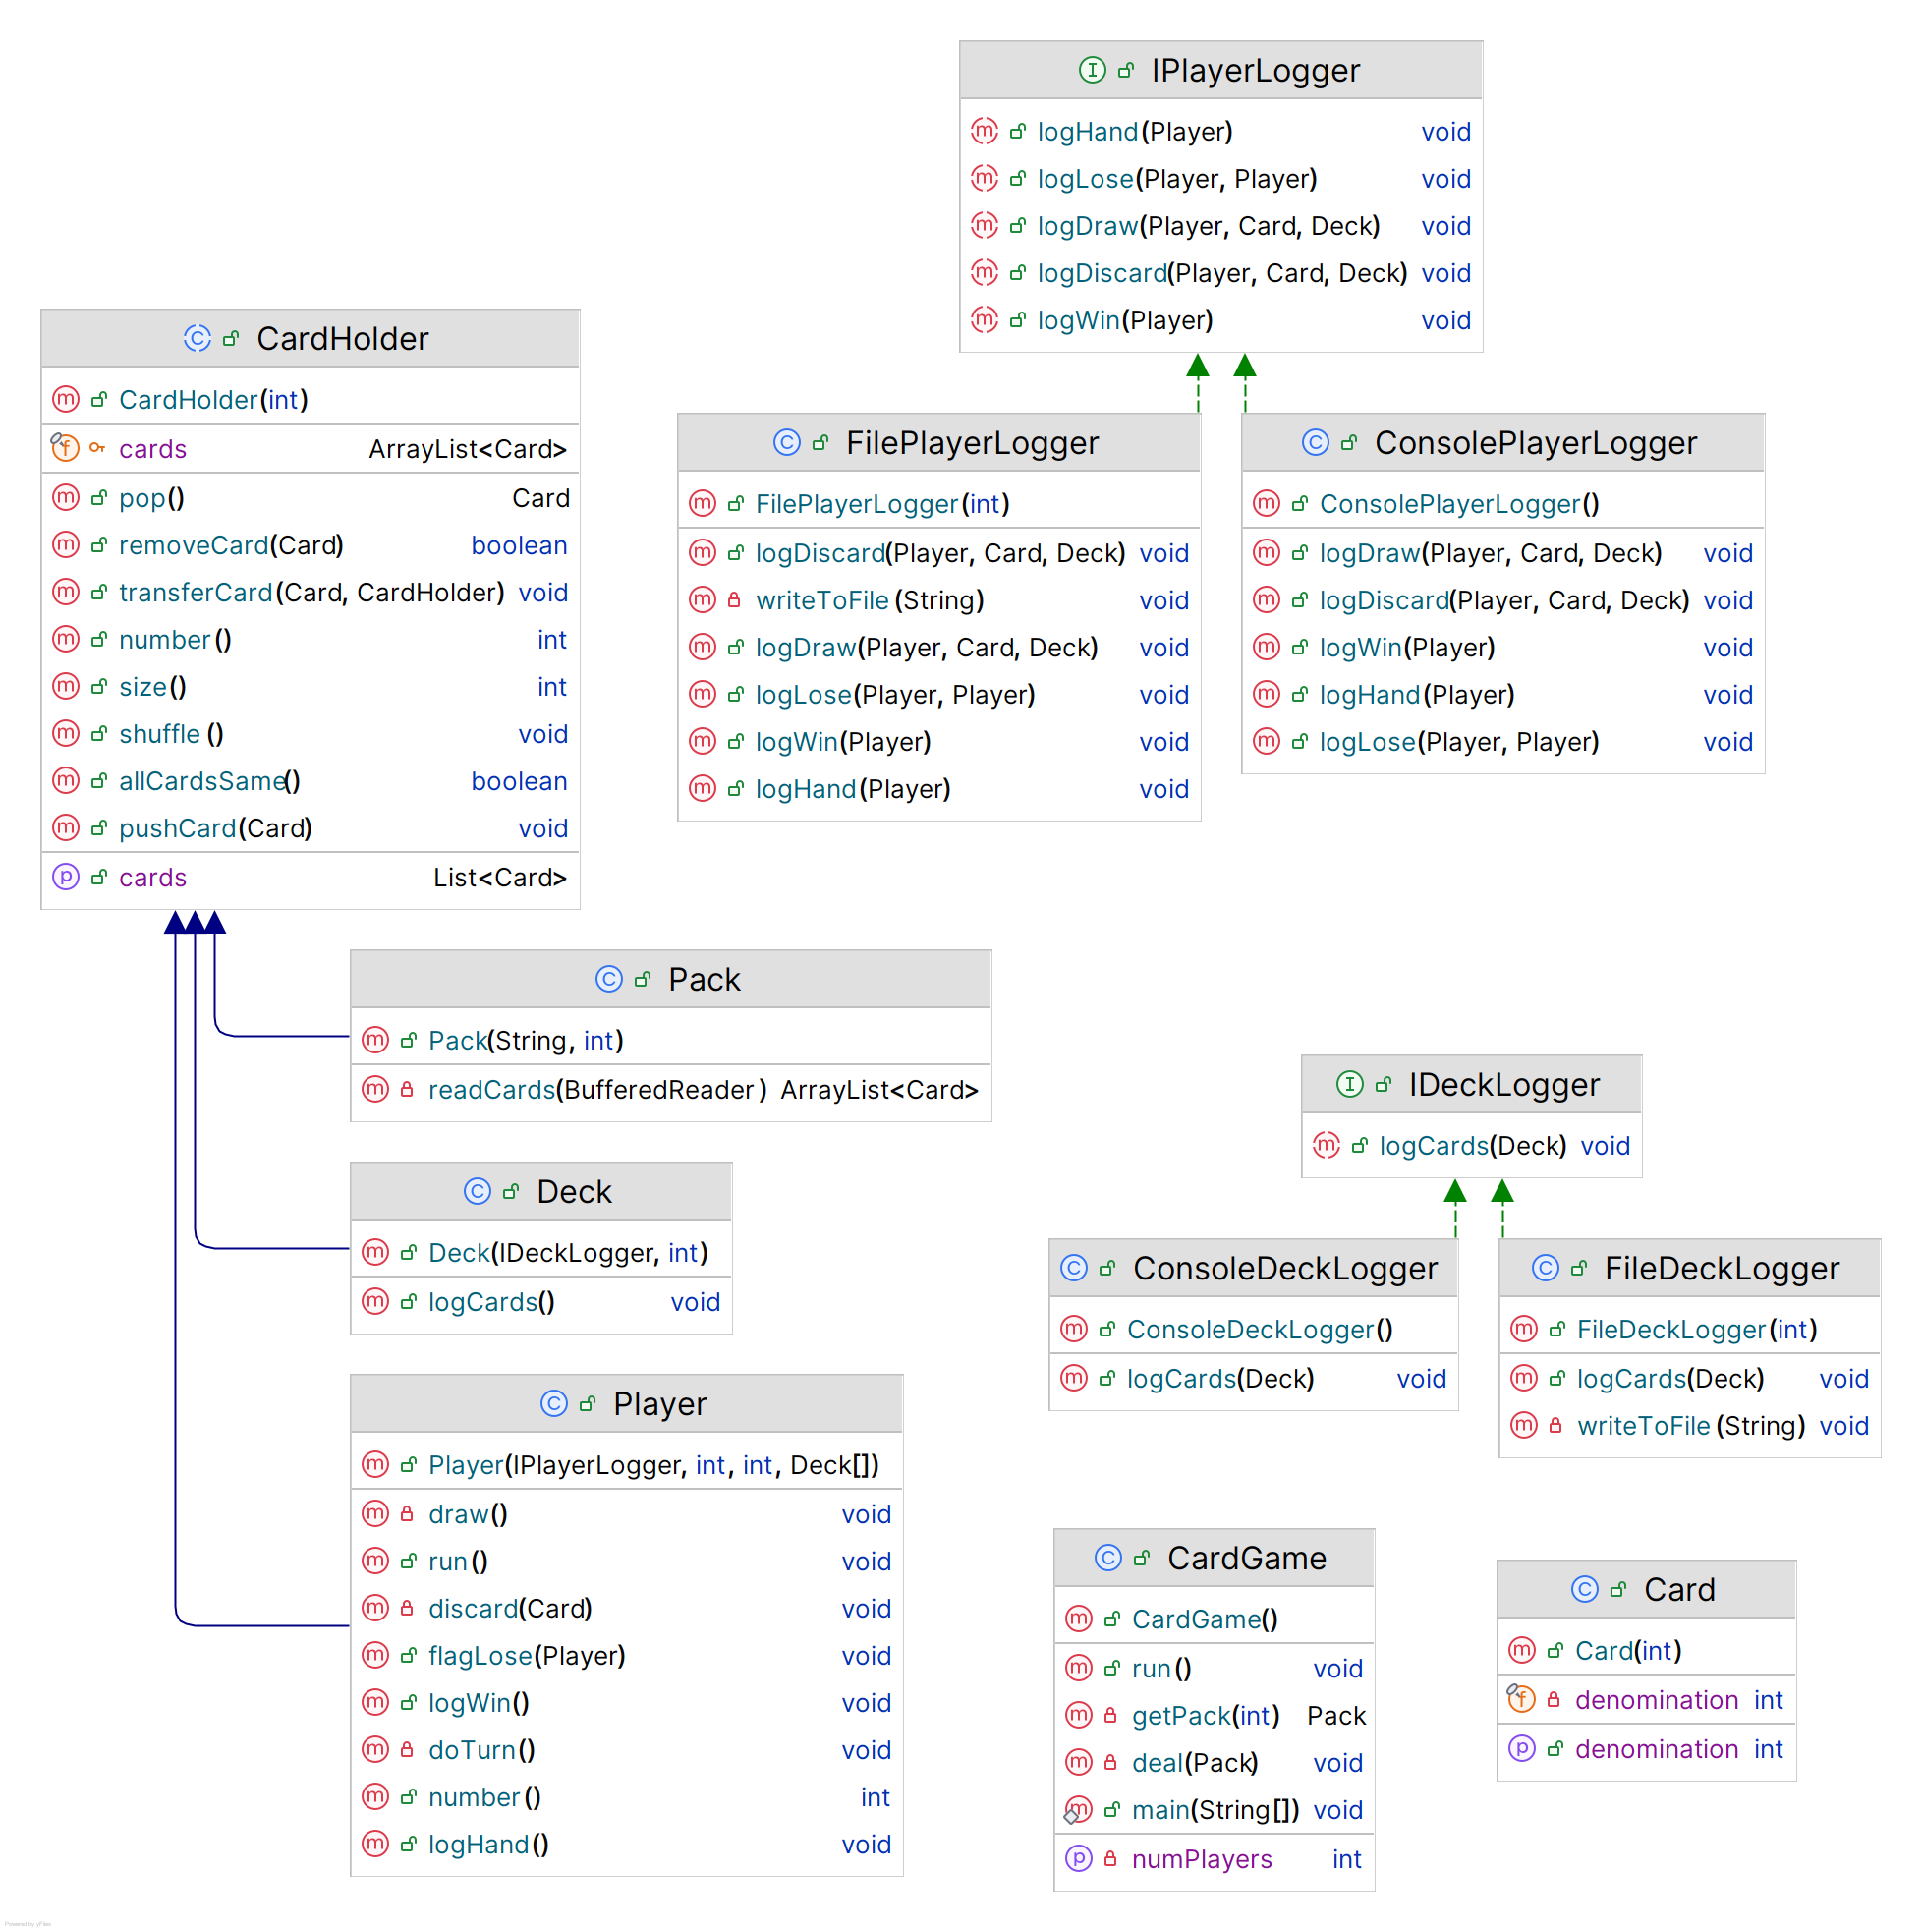
\includegraphics[width=.52\textwidth]{uml}
    \caption{UML Diagram.}
    \label{fig:uml}
\end{wrapfigure}

Benefits of using the V-Model are that:
\begin{enumerate}
    \item It provides a structured approach as phases are completed one at a time.
    \item It is well-suited for pair programming because all requirements are understood by both programmers.
    \item It is simple to understand.
    \item It is easy to manage.
\end{enumerate}
Some drawbacks of the V-Model are that:
\begin{enumerate}
    \item It is not well-suited for large projects.
    \item It is not well-suited for projects with changing requirements.
    \item It is not well-suited for projects with tight deadlines.
\end{enumerate}
Because our project is small and has a fixed set of requirements, the V-Model was well-suited.

The design phase of the V-Model is where we planned the structure of our code and the classes we would need using a UML diagram.

\subsection{UML Diagram}
The UML diagram of our finished production code is shown in Figure~\ref{fig:uml}.

\subsection{Key Design Desicions}
\subsubsection{Facade Design Pattern}
In this UML diagram you can see that we used the facade design pattern to provide a simplified interface to a complex subsystem. The high-level classes like \texttt{IPlayerLogger}, \texttt{IDeckLogger}, and \texttt{CardHolder} act as the facade providing an interface to the underlying subsystems and components.

\subsubsection{The \texttt{CardHolder}}
The abstract class \texttt{CardHolder} is a key part of our design, abstracting common functionality between \texttt{Pack}, \texttt{Deck}, and \texttt{Player}. It implements the following key methods:
\begin{itemize}
    \item \texttt{void pushCard(Card card)}: Adds a card to the \texttt{CardHolder}.
    \item \texttt{void transferCard(Card card, CardHolder target)}: Transfers a card from this \texttt{CardHolder} to another \texttt{CardHolder}.
    \item \texttt{Card pop()}: Removes and returns the top card from the \texttt{CardHolder}.
\end{itemize}
Using an abstract class for this functionality makes it easier for our code to be thread safe, as we can ensure that all operations on a \texttt{CardHolder} are atomic. It also makes testing easier, as we can test the \texttt{CardHolder} class in isolation from the other classes.

\subsubsection{Logging Classes}
Our design uses the interfaces \texttt{IPlayerLogger} and \texttt{IDeckLogger} to provide a common interface for logging player and deck events. This allows us to easily switch between different logging implementations, such as logging to the console or to a file.

This design decision was made to make our code more modular and easier to test. By using interfaces, we can easily mock the logging classes in our tests, allowing us to test the rest of the code in isolation.

It also improved the developer experience, as it made it easier to debug the code with logging being done to the console.

\subsubsection{Separation of Concerns}
Another key point of our design is the separation of concerns. The design separates different responsibilities into distinct classes: \texttt{Pack} is responsible for managing the reading of the pack file, \texttt{Deck} is responsible for managing a deck of cards, and \texttt{Player} is responsible for managing a player's hand.

The benefits of doing this include:
\begin{enumerate}
    \item Easier to test: Each class can be tested in isolation, making it easier to identify and fix bugs.
    \item Easier to maintain: Changes to one class are less likely to affect other classes, making it easier to maintain the codebase.
    \item Easier to understand: Each class has a single responsibility, making it easier to understand the codebase as a whole.
\end{enumerate}

\clearpage
\section{Testing} % Max three pages

\subsection{Design Choices}
Our tests use the JUnit 4 testing framework. We chose JUnit because it is widely used and is well supported in IDEs like IntelliJ IDEA. We used unit tests to test key functionality of our code, such as adding and removing cards from a \texttt{CardHolder}.

Manual system tests were used to test the system as a whole. We tested the system by running the game and checking that the output was as expected. We also tested the system by running the game with different inputs to check that the game behaved correctly in different scenarios.

Our tests used the BICEP testing model. This model is based on testing:
\begin{itemize}
    \item Boundary conditions.
    \item Inverse relationships.
    \item Cross-check results.
    \item Error conditions.
    \item Performance characteristics.
\end{itemize}
We followed the JUnit conventions for test method names, using the format \texttt{test<Method>\_<Scenario>}. This made it easy to identify which method was being tested and what scenario was being tested.

\texttt{assert} methods (\texttt{assertEquals}, \texttt{assertTrue}, etc.) were used to validate the state of the objects being tested.

The \texttt{@Before} annotation was used to create new instances of the classes being tested for each test. This ensured that each test was run in isolation and that the state of the objects being tested was consistent between tests.

\subsection{CardHolderTest}
\subsubsection{Test Coverage}
\begin{itemize}
    \item Testing of \texttt{CardHolder} methods
    \item Tests both successful and edge cases
\end{itemize}
We wanted a range of tests that could test all methods in the \texttt{CardHolder} class effectively and efficiently and follow all the attributes of the Right Bicep test planning model. With that in mind, we designed the tests:
\begin{itemize}
    \item \texttt{pushCard()}
          \begin{itemize}
              \item Tests adding a card to a \texttt{CardHolder}
          \end{itemize}
    \item \texttt{popCard()}
          \begin{itemize}
              \item Tests removing the top card from a \texttt{CardHolder}
          \end{itemize}
    \item \texttt{popCard\_empty()}
          \begin{itemize}
              \item Tests attempting to pop a card from an empty \texttt{CardHolder}
          \end{itemize}
    \item \texttt{removeCard()}
          \begin{itemize}
              \item Tests removing a specific card from a \texttt{CardHolder}
          \end{itemize}
    \item \texttt{removeCard\_nonExistent()}
          \begin{itemize}
              \item Tests removing a card not in the \texttt{CardHolder}
          \end{itemize}
    \item \texttt{transferCard()}
          \begin{itemize}
              \item Tests transferring a card between two Card Holders
          \end{itemize}
    \item \texttt{transferCard\_nonExistent()}
          \begin{itemize}
              \item Tests transferring a non-existent card
          \end{itemize}
    \item \texttt{allCardsSame()}
          \begin{itemize}
              \item Tests checking if all cards in a \texttt{CardHolder} have the same denomination
          \end{itemize}
    \item \texttt{allCardsSame\_empty()}
          \begin{itemize}
              \item Tests \texttt{allCardsSame()} method on an empty \texttt{CardHolder}
          \end{itemize}
    \item \texttt{getCards()}
          \begin{itemize}
              \item Tests retrieving the list of cards from a \texttt{CardHolder}
          \end{itemize}
\end{itemize}

\subsubsection{Error Handling}
\begin{itemize}
    \item We used \texttt{@Test(expected = IllegalStateException.class)} for error scenarios
    \item Verifies correct behaviour when attempting operations on empty collections
\end{itemize}

\subsubsection{State Validation}
\begin{itemize}
    \item Checks list size after operations
    \item Verifies correct card placement and transfer
    \item Ensures state consistency after each operation
\end{itemize}

\subsubsection{Setup Strategy}
\begin{itemize}
    \item We used \texttt{@Before} annotation to create new CardHolder instances for each test
    \item Creates two separate CardHolder instances to test interactions
\end{itemize}

\subsection{CardTest}
Single test method for \texttt{getDenomination()} with basic verification of Card object's core functionality.

\subsection{PackTest}

\subsubsection{Test Coverage}
\begin{itemize}
    \item \texttt{testPackCreation\_ValidFile()}
          \begin{itemize}
              \item Tests creating a Pack with a valid file containing 16 cards
          \end{itemize}
    \item \texttt{testPackCreation\_InvalidFile\_NotEnoughLines()}
          \begin{itemize}
              \item Tests creating a Pack with a file that has insufficient lines
          \end{itemize}
    \item \texttt{testPackCreation\_InvalidFile\_NonIntegerValue()}
          \begin{itemize}
              \item Tests creating a Pack with a file containing a non-integer value
          \end{itemize}
    \item \texttt{testPop\_ValidCase()}
          \begin{itemize}
              \item Tests the \texttt{pop()} method of the Pack - Verifies the first card has the correct denomination (1)
          \end{itemize}
    \item \texttt{testPackCreation\_EmptyFile()}
          \begin{itemize}
              \item Tests creating a Pack with an empty file
          \end{itemize}
\end{itemize}

\subsubsection{File-Based Testing}
\begin{itemize}
    \item We used temporary file creation for testing Pack initialization
    \item Tests multiple file input scenarios
    \item Dynamically generates test files with different contents
\end{itemize}

\subsubsection{Error Scenario Coverage}
\begin{itemize}
    \item Tests pack creation with:
          \begin{itemize}
              \item Valid file
              \item Insufficient lines
              \item Non-integer values
              \item Empty file
          \end{itemize}
\end{itemize}

\subsubsection{File Handling}
\begin{itemize}
    \item Implements a helper method \texttt{createTemporaryPackFile()} to manage test file creation
    \item Uses try-with-resources for safe file writing
    \item We used \texttt{java.nio.file} for temporary file management
\end{itemize}

\clearpage
\section{Work Log}
\begin{table}[H]
    \centering
    \begin{tabular}{llll}
        \toprule
        \textbf{Date} & \textbf{Hours} & \textbf{730022096} & \textbf{730002704} \\
        \midrule
        24/8/24       & 3              & Documentation      & Documentation      \\
        29/10/24      & 3              & Driver             & Observer           \\
        5/11/24       & 3              & Observer           & Driver             \\
        7/11/24       & 2              & Driver             & Observer           \\
        14/11/24      & 4              & Observer           & Driver             \\
        21/11/24      & 4              & Driver             & Observer           \\
        28/11/24      & 3              & Observer           & Driver             \\
        1/12/24       & 4              & Driver             & Observer           \\
        5/12/24       & 4              & Observer           & Driver             \\
        \bottomrule
    \end{tabular}
    \caption{Work Log.}
    \label{tab:work-log}
\end{table}

\end{document}
